%%%%%%%%%%%%%%%%%%%%%%%%%%%%%%%%%%%%%%%%%
% Journal Article
% LaTeX Template
% Version 2.0 (February 7, 2023)
%
% This template originates from:
% https://www.LaTeXTemplates.com
%
% Author:
% Vel (vel@latextemplates.com)
%
% License:
% CC BY-NC-SA 4.0 (https://creativecommons.org/licenses/by-nc-sa/4.0/)
%
% NOTE: The bibliography needs to be compiled using the biber engine.
%
%%%%%%%%%%%%%%%%%%%%%%%%%%%%%%%%%%%%%%%%%

%----------------------------------------------------------------------------------------
%	PACKAGES AND OTHER DOCUMENT CONFIGURATIONS
%----------------------------------------------------------------------------------------

\documentclass[
	a4paper, % Paper size, use either a4paper or letterpaper
	10pt, % Default font size, can also use 11pt or 12pt, although this is not recommended
	unnumberedsections, % Comment to enable section numbering
	twoside, % Two side traditional mode where headers and footers change between odd and even pages, comment this option to make them fixed
]{LTJournalArticle}

\addbibresource{ref.bib} % BibLaTeX bibliography file

\runninghead{DORS with Lazy Constraints} % A shortened article title to appear in the running head, leave this command empty for no running head

\footertext{} % Text to appear in the footer, leave this command empty for no footer text

\setcounter{page}{1} % The page number of the first page, set this to a higher number if the article is to be part of an issue or larger work

%----------------------------------------------------------------------------------------
%	TITLE SECTION
%----------------------------------------------------------------------------------------

\title{Distributed Operating Room Scheduling using Lazy Constraints and Networks} % Article title, use manual lines breaks (\\) to beautify the layout

% Authors are listed in a comma-separated list with superscript numbers indicating affiliations
% \thanks{} is used for any text that should be placed in a footnote on the first page, such as the corresponding author's email, journal acceptance dates, a copyright/license notice, keywords, etc
\author{%
	Ethan Merrick\textsuperscript{1}, Benjamin Solomon\textsuperscript{1} and Mitchell Clark\textsuperscript{1}
}

% Affiliations are output in the \date{} command
\date{\footnotesize\textsuperscript{\textbf{1}}The University of Queensland}

% Full-width abstract
\renewcommand{\maketitlehookd}{%
	\begin{abstract}
		\noindent 
		We re-implemented existing models\cite{roshanaei2017propagating} for solving the distributed operating room scheduling (DORS) problem. We extend the existing formulation with a new LBBD cut, we extend the implementation by employing lazy constraints in Gurobi and we try a network model formulation. We were not able to replicate results inline with the original paper. It was found that... <TO BE CONTINUED>. % Add comment about results.
	\end{abstract}
}

% \documentclass[10pt, reqno]{amsart}
% % \documentclass[aps,twocolumn,secnumarabic,balancelastpage,amsmath,amssymb,nofootinbib,floatfix]{article}
\usepackage{setspace,tikz,xcolor,mathrsfs,listings,multicol, amsmath, amssymb}
\usepackage{rotating}
\usepackage{float, siunitx}
\usepackage[section]{placeins}
\usepackage{caption}
\usepackage{subcaption}
%\usepackage{fullpage}
% \usepackage[all,cmtip]{xy}
% \usetikzlibrary{arrows,matrix}
% \usepackage[margin=1.25in]{geometry}

% % \onehalfspacing

% \usepackage[colorlinks=true, pdfstartview=FitV, linkcolor=blue, citecolor=blue, urlcolor=blue]{hyperref}

% % For breaking equations across multiple pages
% % \allowdisplaybreaks[1]
% \usepackage[colorinlistoftodos]{todonotes}
% \setlength\marginparwidth{1in}
% \newcommand{\ethan}[1]{\todo[size=\tiny,color=red!30]{#1 \\ \hfill --- Travis}}
% \newcommand{\Ethan}[1]{\todo[size=\tiny,inline,color=red!30]{#1
% 		\\ \hfill --- Travis}}
% \newcommand{\mitchell}[1]{\todo[size=\tiny,color=blue!30]{#1 \\ \hfill --- Mitchell}}
% \newcommand{\Mitchell}[1]{\todo[size=\tiny,inline,color=blue!30]{#1
% 		\\ \hfill --- Mitchell}}
% \newcommand{\benjamin}[1]{\todo[size=\tiny,color=green!30]{#1 \\ \hfill --- Benjamin}}
% \newcommand{\Benjamin}[1]{\todo[size=\tiny,inline,color=green!30]{#1
% 		\\ \hfill --- Benjamin}}



%%%%%%%%%%%%%%%%%%%%%%%%%%%%%%%%%%%%%%%%

\begin{document}
	% \title[]{The Proj}
	
	% \author[M.~Clark]{Mitchell Clark}
	% \author[B.~Solomon]{Benjamin Solomon}
    % \author[E.~Merrick]{Ethan Merrick}
	
	% \keywords{operations research}
	% \subjclass[2010]{}

	
	
	% \begin{abstract}
		
	% \end{abstract}

	\maketitle
	% % \twocolumn
	% \setcounter{tocdepth}{1}
	% \tableofcontents
	\section{Introduction}
	Our report is based upon~\cite{roshanaei2017propagating} which we will also refer to as \textit{the original paper} throughout. The paper solves the deterministic distributed  operating room scheduling (DORS) problem using Logic-Based Benders' Decomposition (LBBD) and a cut propagation method. This formulation has been extended upon in a stochastic setting\cite{guo}. We re-implemented the paper and extended the formulation with a new LBBD cut and a network model. We extended implementation by using lazy constraints in Gurobi. Our main goals were to replicate the results found in the original paper and investigate if there was potential improvement to be had by using lazy constraints instead of iteration.

% Structure scale and extendability of original models
The LBBD framework outlined in~\cite{roshanaei2017propagating} is structured as a location-allocation master problem with a bin-packing sub problem simplified by symmetric operating rooms. The results in the original paper show that the proposed models scale well for up to 160 patients.

% Overview of models in OG paper
The original paper contains many variants of models, they provide a pure MIP formulation, and an LBBD formulation with three different types of cuts. For each of these cuts they experiment with a version with and without propagation. For each of these they implement different cut generation schemes which determine how many sub problems to iterate over before re-solving the master problem. We choose some of their models to best achieve our goals. We choose to use the maximal cut generation scheme, iterating over all sub-problems before re-solving the master problem.

% DORS Problem definition.
In the DORS problem, we seek to decide which hospital operating suites and their respective operating rooms to open. We also decide which patients to allocate to each hospital day. We make these decisions in such a way as to minimize the the total cost of opening facilities while also trying to maximize the reward for assigning critical patients\cite{roshanaei2017propagating}.
	\section{Model Formulation}
	\subsection{Master Problem} 

The following is the LBBD formulation of the problem.
For a pure IP formulation refer to \cite{roshanaei2017propagating}. We will first outline
the formulation of the master problem. The master problem handles assignment of patients
to hospital-days.

\begin{table}[H]
% \captionsetup{font={Large,sf}}
\caption*{\bf{SETS}}
\resizebox{0.45\textwidth}{!}{
\begin{tabular}{ll}
    $\mathcal{P}$ &  Set of patients $p \in \mathcal{P}$\\
    $\mathcal{P}{'} $ & Set of mandatory patients, $\mathcal{P}{'} = \lbrace p|\rho_{p}(|\mathcal{D}|-\alpha_{p})\leq-\Gamma\rbrace$\\
    $\mathcal{H} $ & Set of hospitals, $h \in \mathcal{H}$\\
    $\mathcal{D} $ & Set of days in the planning horizon, $d \in \mathcal{D}$\\
    $\mathcal{R}_{h} $ & Set of ORs in each hospital's surgical suite, $r \in \mathcal{R}_{h}$\\
\end{tabular}
}

\end{table}

\begin{table}[H]
\caption*{\bf{DATA}}
\label{tab:MPdata}
\resizebox{0.45\textwidth}{!}{
\begin{tabular}{ll}
    $G_{hd}$ & Cost of opening the surgical suite in hosptial h on\\
    &  $\quad$ day d.\\
    $F_{hd} $ & Cost of opening and OR in hospital h on day d. \\
    $B_{hd} $ & Regular operating hours of each OR on day d. \\
                & $\quad$ in hospital h.\\
    $T_{hp} $ & Total booked time (preparation time + surgery time\\
               & $\quad$ + cleaning time) of patient p.\\
    $\rho_{p} $ & Health status score assigned to patient p.\\
    $\alpha_{p} $ & Number of days elapsed from the referal date of \\
    & $\quad$ patient p.\\
    $\kappa_{1} $ & Waiting cost for scheduled patients.\\
    $\kappa_{2} $ & Waiting cost for unscheduled patients.\\
    $\Gamma $ & Health status threshold above which patients have to\\
    & $\quad$ be operated.
\end{tabular}
}
\end{table}
\begin{table}[H]
\caption*{\bf{VARIABLES}}
\label{tab:MPvariables}
\resizebox{0.45\textwidth}{!}{
\begin{tabular}{ll}
    $x_{hdp} $ & 1 if patient p is assigned to hospital h on day d\\
    & $\quad$, 0 otherwise\\
    $u_{hd} $ & 1 if the surgical suite in hospital h is opened\\
    & $\quad$ on day d, 0 otherwise\\
    $y_{hd} $ & $\in \mathbb{Z}^+$,  lower bound on number of operating rooms \\
    & $\quad$ open in hospital h on day d \\
    $w_{p}$ & 1 if patient p is not scheduled this horizon,\\
    & $\quad$ 0 otherwise\\ 
\end{tabular}
}
\label{MP:variables}
\end{table}
\leavevmode
% \newline
% %setting up the master problem
\subsubsection*{Objective}

The objective function balances the minimisation of costs associated with opening hospitals
 and ORs and maximising the reward of assigning patients to surgeries. 
\begin{align}
\operatorname{minimize} \bigg( &\sum\limits_{h \in \mathcal{H}} \sum\limits_{d \in \mathcal{D}} G_{hd} U_{hd} 
 + \sum\limits_{h \in \mathcal{H}}\sum\limits_{d \in \mathcal{D}} F_{hd} y_{hd} \label{eq:MPobjective}
\\ &+ \sum\limits_{h \in \mathcal{H}} \sum\limits_{d \in \mathcal{D}} \sum\limits_{p \in \mathcal{P}}  
\kappa_{1} [\rho_{p} (d - \alpha_{p}) x_{hdp}]\notag
\\ &+ \sum\limits_{p \in \mathcal{P} \setminus \lbrace \mathcal{P}{'} \rbrace } \kappa_{2} [\rho_{p}( \mathcal{D} + 1 -\alpha_{p} ) w_{p}]
\bigg) \notag
\end{align}

\subsubsection*{Constraints} The constraints for the MP are formulated as follows.
\begin{align}
    \sum\limits_{h \in \mathcal{H}} \sum\limits_{d \in \mathcal{D}}x_{hdp} = 1 
        && \forall p \in \mathcal{P}' \label{MPcon1}\\
    \sum\limits_{h \in mathcal{H}} \sum\limits_{d \in \mathcal{D}} x_{hdp} + w_p = 1
        && \forall p \in \mathcal{P} \backslash \{\mathcal{P}'\}\label{MPcon2}\\
    x_{hdp} \leq u_{hd}
        && \forall h \in \mathcal{H}, d \in \mathcal{D}, p \in \mathcal{P}\label{MPcon3}\\
    \sum\limits_{p \in \mathcal{P}}T_px_{hdp} \leq |\mathcal{R}_h|B_{hd}u_{hd}
        && \forall h \in \mathcal{H}, d \in \mathcal{D} \label{MPcon4}\\
    T_p\,x_{hdp} \leq B_{hd} 
        && \forall h \in \mathcal{H}, d \in \mathcal{D}, p \in \mathcal{P}\label{MPcon5}\\
     \sum_{p \in \mathcal{P}}T_px_{hdp} \leq B_{hd}y_{hd}
        && \forall h \in \mathcal{H}, d\in \mathcal{D} \label{MPcon6}\\
        y_{hd} \leq |\mathcal{R}_h|
        && \forall h\in\mathcal{H}, d \in \mathcal{D} \label{MPcon7}\\
        u_{hd}, x_{hdp} \in \{ 0,1\}
        && \forall h\in \mathcal{H}, d \in \mathcal{D}, p \in \mathcal{P}\label{MPcon8}\\
        w_p \in \{0,1\}
        && \forall p \in \mathcal{P} \backslash\{\mathcal{P}'\}\label{MPcon9}
\end{align}
Constraint (\ref{MPcon1}) ensures all mandatory patients are assigned in the planning 
horizon. Constraint (\ref{MPcon2}) ensures that variables $x_{hdp}$ and $u_{hd}$ are not
turned on simultaneously. Constraint (\ref{MPcon3}) ensures that if a patient is assigned
a hospital-day then that hospital-day is open. (\ref*{MPcon4}) ensures that surgery time 
of patients assigned to a hospital-day does not exceed the available surgery time in
that hospital day. (\ref*{MPcon5}) ensures an individuals surgery time does not exceed 
the hospital-day's available time. (\ref*{MPcon6}) ensures $y_{hd}$ gives a lower bound 
on the number of operating rooms. (\ref*{MPcon7}) ensures $y_{hd}$ does not exceed the
number of operating rooms available on a hospital-day. Constraints (\ref*{MPcon8}) -- (\ref*{MPcon9}) simply restrict
variables to binary.

\subsection{Subproblems}
Given a solution to the master problem $(\widehat{Y}^{(i)}_{hd}, \widehat{\mathcal{P}}^{(i)}_{hd})$ the 
subproblem minimises the number of ORs to open for a given hospital day. Each subproblem is
formulated as follows.

\begin{table}[H]
    \caption*{\bf{ADDITIONAL VARIABLES}}
    \resizebox{0.45\textwidth}{!}{
        \begin{tabular}{ll}
            $y_r$ & $\in \mathbb{Z}^+$, number of open operating rooms. \\
            $x_{pr}$ & 1 if patient p is assigned to operating room r,\\
            &   $\quad$ 0 otherwise.
        \end{tabular}
    }
\end{table}
\begin{align}
    \operatorname*{minimise} \quad \overline{Y}_{hd} = \sum\limits_{r \in \mathcal{R}_h}y_r
\end{align}

With constraints given as follows:
\begin{align}
    \sum\limits_{r\in\mathcal{R}_h}x_{pr} = 1 && \forall p \in \widehat{\mathcal{P}}^{(i)}_{hd}\label{SPcon1}\\
    \sum\limits_{p \in \widehat{\mathcal{P}}^{(i)}_{hd}} T_px_{pr} \leq B_{hd}y_r 
    && \forall r \in \mathcal{R}_h \label{SPcon2}\\
    x_{pr} \leq y_r && \forall p \in \widehat{\mathcal{P}}^{(i)}_{hd}, r \in \mathcal{R}_h \label{SPcon3}\\
    y_r \leq y_{r-1} && \forall r \in \mathcal{R}_h \backslash \{1\}\label{SPcon4}\\
    x_{pr},\,y_r\in\{0,1\} && \forall p \in \widehat{\mathcal{P}}^{(i)}_{hd}, r \in \mathcal{R}_h\label{SPcon5}
\end{align}
Constraint (\ref*{SPcon1}) ensures that each patient is assigned to only one operating room.
Constraint (\ref*{SPcon2}) ensures that no OR is overcapacitated. Constraint (\ref*{SPcon3})
ensures that patients are assigned to open ORs. Constraint (\ref*{SPcon4}) breaks symmtry
among ORs.

\subsection{Benders Cuts}
There are multiple forms of benders cuts outlined in the original paper. We will discuss
pertinent forms based on their performance as discussed in the original paper. These are 
the LBBD1 and LBBD2 benders cuts. In order to describe these cut types, we will first discuss the 
first-fit decreasing heuristic algorithm (FFD) as this is used to determine optimality of SPs. 

\subsubsection*{First-fit decreasing heuristic algorithm}
Since the SP packing problem can be difficult to solve, we can first find a feasible solution 
($\overline{F}^{(i)}_{hd}$) using a FFD heuristic. This process is faster than other techniques
such as integer and constraint programming. Moreover, we have the following relationship 
between the FFD, MP and SP solutions;
\begin{equation}
    \tilde{Y}^{(i)}_{hd} \leq \overline{Y}^{(i)}_{hd} \leq \overline{F}^{(i)}_{hd}
\end{equation}
We can use the FFD solution $\left(\overline{F}^{(i)}_{hd}\right)$ to find an optimal SP solution 
$\left(\overline{Y}^{(i)_{hd}}\right)$ without explicitly solving the SP. Moreover, if 
$\overline{F}^{(i)}_{hd} \neq \tilde{Y}^{(i)}_{hd}$ then when solving the SP we can use 
$\operatorname{min}\{\overline{F}^{(i)}_{hd},\, |\mathcal{R}_h|\}$ as an upper bound. 

\subsubsection{LBBD1}
LBBD1~\cite{roshanaei2017propagating} utilises both feasibility and optimality cuts to 
correct the MP to find a solution. If the SP is infeasible the following "no good" cut 
is added to the MP which requires at least one patient be removed from 
$\tilde{\mathcal{P}}^{(i)}_{hd}$.
\begin{align}
    \sum\limits_{p \in \tilde{\mathcal{P}}^{(i)}_{hd}}(1-x_{hdp})\geq 1 
        && \forall (h,d) \in \mathcal{U}_{hd}^{(i)}
\end{align}
Where $\mathcal{U}_{hd}^{(i)}$ is the set of infeasible SPs at this stage of solving the MP.
If the SP is optimal, that is $\tilde{Y}^{(i)}_{hd} = \overline{Y}^{(i)}_{hd}$, no cuts
are required. However, if the this is not the case, the following optimality cut is added:
\begin{align*}
    y_{hd} \geq \overline{Y}_{hd}^{(i)} - \sum\limits_{p \in \hat{\mathcal{P}}}(1-x_{hdp}) && \forall (h,d) \in \overline{\mathcal{J}}^{(i)}.
\end{align*}
Where $\overline{\mathcal{J}}^{(i)}$ is the set of SPs that are not optimal at a particular stage of solving the MP. This cut effectively has two results. It either forces at least one more OR open, or removes one patient from $\tilde{\mathcal{P}}^{(i)}_{hd}$.
\subsubsection{LBBD2}
LBBD2 differs from LBBD1 in its feasibility cut which is given as follows:
\begin{align*}
    y_{hd} \geq (|\mathcal{R}_h| + 1) - \sum\limits_{p \in \hat{\mathcal{P}}_{hd}^{(i)}}(1-x_{hdp}) && (h,d) \in \overline{\mathcal{U}}^{(i)}.
\end{align*}
If $\overline{Y}_{hd}^{(i)} = |\mathcal{R}_h|$ and the SP is infeasible then this cut simply removes one patient from $\overline{\mathcal{P}}_{hd}^{(i)}$. However, if $\hat{Y}_{hd}^{(i)} \le |\mathcal{R}_h|$ and the SP is infeasible then the cut either removes two patients from $\overline{\mathcal{P}}_{hd}^{(i)}$, or removes one patient and/or opens at least one more OR.
\subsubsection{Cut Propagation}
The original paper utilises cut propagation for LBBDs in order to generate multiple cuts for each infeasible SP. This is done by recognising that an infeasible set of patients for a particular hospital-day cannot be packed into a hospital-day with less or equal OR time.
\subsection{Network Problem}
We also give the formulation of the problem as a network. The problem contains the sets
and data of the master problem previously outlined with the addition of the following 
sets and data. Nodes represent hospital-day-time, where time is in minute intervals. Arcs represent assignment of patients to operating rooms.
\begin{table}[H]
    % \captionsetup{font={Large,sf}}
    \caption*{\bf{SETS}}
    \resizebox{0.4\textwidth}{!}{
    \begin{tabular}{ll}
        $\mathcal{N}$ &  Set of nodes $n \in \mathcal{N}$ for each hospital-day-minute\\
        $\mathcal{N^\prime}$ & Set of nodes $n \in \mathcal{N}$ \\
        & $\operatorname{s.t.} \operatorname{minDur} \leq n[time] \leq B_{n[time],n[day]} - \operatorname{minDur} $ \\
        $\mathcal{A}$ &  Set of arcs $a \in \mathcal{A}$ between nodes $n \in N$\\
    \end{tabular}
    }
    \end{table}
    \begin{table}[H]
        % \captionsetup{font={Large,sf}}
        \caption*{\bf{DATA}}
        \resizebox{0.45\textwidth}{!}{
        \begin{tabular}{ll}
            $t_n$ & Arcs that enter node $n \in \mathcal{N}$ \\
            $f_n$ & Arcs that leave node $n \in \mathcal{N}$\\
            $h_a$ & Hospital associated with arc $a \in \mathcal{A}$\\
            $d_a$ & Day associated with arc $a \in \mathcal{A}$ \\
            $\operatorname{patient}_a$ & Patient associated with arc $a \in \mathcal{A}$\\
            $\operatorname{start}_a$ & Start time of arc $a \in \mathcal{A}$\\
            $\operatorname{end}_a$ & End time of arc $a \in \mathcal{A}$\\
            $\operatorname{minDur}$ & minimum surgery duration 
        \end{tabular}
        }
        \end{table}
    The variables are also shared with the master problem with the addition of the following variable. 
\begin{table}[H]
    \caption*{\bf{VARIABLES}}
    \label{tab:NETvariables}
    \resizebox{0.4\textwidth}{!}{
    \begin{tabular}{ll}
        $z_{a}$ & 1 if arc a is turned on, 0 otherwise.
    \end{tabular}
    }
    \end{table}

    \subsubsection*{Objective}
    The objective function is identical to master problem objective given in \ref{eq:MPobjective}.
    \begin{align}
    \operatorname{minimize} \bigg( &\sum\limits_{h \in \mathcal{H}} \sum\limits_{d \in \mathcal{D}} G_{hd} U_{hd} 
     + \sum\limits_{h \in \mathcal{H}}\sum\limits_{d \in \mathcal{D}} F_{hd} y_{hd}
    \\ &+ \sum\limits_{h \in \mathcal{H}} \sum\limits_{d \in \mathcal{D}} \sum\limits_{p \in \mathcal{P}}  \label{MP:objective}
    \kappa_{1} [\rho_{p} (d - \alpha_{p}) x_{hdp}]
    \\ &+ \sum\limits_{p \in \mathcal{P} \setminus \lbrace \mathcal{P}{'} \rbrace } \kappa_{2} [\rho_{p}( \mathcal{D} + 1 -\alpha_{p} ) w_{p}]
    \bigg) \notag
    \end{align}
    
    \subsubsection*{Constraints} The constraints for the network formulation are given as follows,
    \begin{align}
        \sum\limits_{a \in f_n} z_a = \sum\limits_{a \in t_n} z_a 
            && \forall n \in \mathcal{N}^\prime \label{NETcon1:room_flow}\\
        \sum\limits_{\substack{a \in \mathcal{A} | \\ (h_a, d_a, \operatorname{start}_a) \\= (h,d,0)}}z_a \leq y_{hd}
            && \forall d \in \mathcal{D} \forall h \in \mathcal{H}\label{NETcon2:restrict_ops_by_ors}\\
        \sum\limits_{\substack{a \in \mathcal{A} |\\ (h_a,d_a,\operatorname{patient}_a)\\ =(h,d,p)}}z_a= x_{hdp}
            && \forall h \in \mathcal{H}, \forall d \in \mathcal{D}, \forall p \in \mathcal{P}  \label{NETcon3:is_patient_operated_on} \\
        \sum\limits_{h \in \mathcal{H}} \sum\limits_{d \in \mathcal{D}}x_{hdp} = 1 
            && \forall p \in \mathcal{P}' \label{NETcon4:must_do_mandatory}\\
        \sum\limits_{h \in \mathcal{H}} \sum\limits_{d \in \mathcal{D}} x_{hdp} + w_p = 1
            && \forall p \in \mathcal{P} \backslash \{\mathcal{P}'\}\label{NETcon5:turn_on_w}\\
        x_{hdp} \leq u_{hd}
            && \forall h \in \mathcal{H}, d \in \mathcal{D}, p \in \mathcal{P}\label{NETcon5:force_hosp_on}\\
            y_{hd} \leq |\mathcal{R}_h|
            && \forall h\in\mathcal{H}, d \in \mathcal{D} \label{NETcon6:max_OR}\\
            u_{hd}, x_{hdp} \in \{ 0,1\}
            && \forall h\in \mathcal{H}, d \in \mathcal{D}, p \in \mathcal{P}\label{con8}\\
            w_p \in \{0,1\}
            && \forall p \in \mathcal{P} \backslash\{\mathcal{P}'\}\label{con9}
    \end{align}
    Constraint

    Constraint (\ref{con1}) ensures all mandatory patients are assigned in the planning 
    horizon. Constraint (\ref{con2}) ensures that variables $x_{hdp}$ and $u_{hd}$ are not
    turned on simultaneously. Constraint (\ref{con3}) ensures that if a patient is assigned
    a hospital-day then that hospital-day is open. (\ref*{con4}) ensures that surgery time 
    of patients assigned to a hospital-day does not exceed the available surgery time in
    that hospital day. (\ref*{con5}) ensures an individuals surgery time does not exceed 
    the hospital-day's available time. (\ref*{con6}) ensures $y_{hd}$ gives a lower bound 
    on the number of operating rooms. (\ref*{con7}) ensures $y_{hd}$ does not exceed the
    number of operating rooms available on a hospital-day. Constraints (\ref*{con8}) -- (\ref*{con9}) simply restrict
    variables to binary.
	\section{Data}
	test
	\section{Implementation}
	% Specs and general overview
Models were run on a Windows 11 computer with a AMD Ryzen 5 5625U 2.3GHz processor with 16 GB of RAM\@. Gurobi version 10.0.1 was used with Python version 3.9.16. We implemented two different models for LBBD, one following\cite{roshanaei2017propagating} which solves the master problem iteratively in a loop, rebuilding the master problem branch-and-bound tree on every iteration. The other model leveraged lazy constraints in Gurobi to perform a branch and check routine\cite{LBBDBible}, building the branch-and-bound tree once while applying Benders' cuts as lazy constraints at each new incumbent solution. The pure MIP and network model were solved using standard Gurobi routines. 

% Implementation difficulty
Model formulations were simple enough to interpret but practical implementation was difficult for a few reasons. Firstly, the original paper did not supply any code. This made it hard to find implementation details that may have drastically improved results, for example some important caching protocol may have been used that was not mentioned in the paper. Further, the paper supplied distribution parameters that were useful in generating data, however it did not supply the data instances that were used to generate their results. This made it impossible to verify if the differences seen in our results were due to an implementation error, random chance or something else. It also left data inadequately described. For example the surgery times were said to be from a normal distribution, this might imply that they should be real-valued. However, upon inspection of another paper's data which worked on a similar problem\cite{guo}, it was noticed that surgery times were rounded to some integer value. Implementing this with our data generation scheme immediately improved the performance of our models. We reached out to the author of the original paper and we were told that they were no longer in possession of either the code or data that was used. 

The paper did not supply example objective values found for their instances which made it hard to determine feasibility of our solutions. Ultimately the main verification method of our results was by the consistency of outputted optimal objective values across all models implemented. That is, the pure MIP, Network and Benders' models were implemented in sufficiently different ways but all provided the same output giving us some level of confidence in our implementation's optimality. Feasibility was verified by manual inspection of patient allocations for instances with small number of patients. We had no way of verifying if the speed of our models would be the same as achieved by the models used in the original paper.
	\section{Results}
	% Runtime specifications
Models were run on a Windows 11 computer with an AMD Ryzen 5 5625U 2.3GHz processor with 16 GB of RAM\@. Gurobi version 10.0.1 was used with Python version 3.9.16. 

We aimed to compare 7 models: The pure MIP, the network model, an iterative LBBD1 (iLBBD1), LBBD1 using lazy constraints (cLBBD1), iterative LBBD2 with propagation (iLBBD2p), LBBD2 with lazy constraints and propagation (cLBBD2p) and LBBD4 with lazy constraints and propagation (cLBBD4). The pure MIP was used as a baseline.\ iLBBD1 and cLBBD1  were chosen to be used as baseline LBBD models. LBBD2 with propagation was chosen as it was one of the best performers in the original paper, we intended to use it as the main comparison to the network model and our new cut. We chose to collect results for LBBD4 only using propagation and lazy constraints as we believed this would give us the best results while adhering to the project time constraints.

We generate 5 seeded instances of data similarly to~\cite{roshanaei2017propagating}. The data is generated for 3 hospitals and 5 operating rooms over a 5 day planning horizon for varying number of patients. Unlike~\cite{roshanaei2017propagating} who generate a set of data for 3 and 5 operating rooms while only varying the surgery times in each instance, we generate each instance with entirely different data. This was believed to give results more indicative of performance on a wider variation in problem parameters. Also unlike in the original paper, where models were ran with a time limit of 7200 seconds, we set our time limit to 900 seconds due to project time constraints. At a time limit of 7200 seconds the worst case time to run all models over all 5 instances was 70 hours for only one patient size. For this same reason we only ran models with 5 available operating rooms, instead of testing both 5 and 3. We chose to use 5 operating rooms, this should have led to harder sub problems and relatively easier master problems compared to using 3 operating rooms\cite{roshanaei2017propagating}. 

There was uncertainty as to whether the models were solved to true optimality or to a relative MIP gap of $1\%$ as was done by~\cite{guo}, so we report results for both scenarios. We follow~\cite{roshanaei2017propagating} by defining the best performing model to be the most robust, that is, the one able to solve the model to optimality within the given time constraints while breaking ties by considering the fastest models averaged over solved instances.

The 7 models were solved to optimality on each of the 5 instances, the average time to solve can be seen in Table~\ref{tab:avgTimeOpt} and the average gaps can be seen in Table~\ref{tab:avgGapOpt}.

\begin{table*}
    \centering
    \caption{Average time (seconds) until solved to optimality over 5 instances. The number of instances not solved to optimality are superscripted. Non-solved instances are not included in average. **** represents that no instances solved in time.}
    \begin{tabular}{rrrrrrrr} \toprule
        $|\mathcal{P}|$ & Pure MIP & Network & iLBBD1 & cLBBD1 & iLBBD2p & cLBBD2p & cLBBD4p \\ \midrule
        20              & 16.06 &     ${****}^{(5)}$    & 1.509 &  0.8829 & 1.431 & 0.8800 & 0.7890 \\
        40              & $179.3^{(2)}$ & $268.5^{(3)}$   &  $4.429$ & $1.911^{(4)}$ & $4.503^{(1)}$ & $1.911^{(4)}$ & $1.959^{(4)}$ \\
        60 & $30.80^{(4)}$ & ${****}^{(5)}$ & $24.46^{(1)}$ & $10.73^{(4)}$ & $34.61^{(2)}$ & $21.46^{(4)}$ & $25.80^{(4)}$ \\
        80 & ${****}^{(5)}$ & ${****}^{(5)}$ & ${****}^{(5)}$ & ${****}^{(5)}$ & ${****}^{(5)}$ & ${****}^{(5)}$ & ${****}^{(5)}$ \\
        \bottomrule
    \end{tabular}
\end{table*}


We can see from Table~\ref{tab:avgTimeOpt} that all models struggled solving to optimality for number of patients greater than only 20. The pure MIP was the most robust across all patient sizes while the Network model was the least. We can see that for sizes where LBBD models do solve an instance, they do so on average faster than the pure MIP.\@ For example, for a patient size of 20 cLBBD4p performed the best, being solved in the least time on average, with cLBBD2p being close second. For a patient size of 60, most LBBD models solved faster than the pure MIP.\@ Comparing between LBBD models, all using lazy constraints outperform those using iteration in terms of time to solve for every number of patients. The results shown in Table~\ref{tab:avgTimeOpt} suggest that none of the 7 models scale well for solving problems with sets of patients as large or larger than 60 when solving to optimality. No models were able to solve instances with 80 patients to optimality. 

\begin{table*}
    \centering
    \caption{Average gap (\%) over 5 instances after trying to solve to optimality. MIPGap is reported for pure MIP, Network and callback implementations of LBBD.\@ Gap between master problem lowerbound and best sub problem upperbound is report for iterative implementations of LBBD.}\label{tab:avgGapOpt}
    \begin{tabular}{rrrrrrrr} \toprule
        $|\mathcal{P}|$ & Pure MIP & Network & iLBBD1 & cLBBD1 & iLBBD2p & cLBBD2p & cLBBD4p \\ \midrule
        20              & 0.000 &    $0.4950$     & 0.000 &  0.000 & 0.000 & 0.000 & 0.000 \\
        40              & $0.04220$ & $0.3382 $  & $0.6252 $ & $0.3532 $ & $0.09500 $ & $0.4765 $ & $0.4948$ \\
        60 & $0.1827 $ & $0.4131 $ & $0.5514 $ & $0.2540 $ & $0.1700 $ & $0.3513 $ & $0.3273 $ \\
        80 &  $0.2630 $ &  $0.2048 $ & $0.9390$ &  $0.6000 $ & $0.2100$ & $0.4718 $ & $0.5218$ \\
        \bottomrule
    \end{tabular}
\end{table*}


Table~\ref{tab:avgGapOpt} shows that although not many instances solved to optimality, by the end of the prescribed time limit, the optimality gaps were very small. All optimality gaps had reached at least 1\% or lower. In fact, increasing the number of patients did not appear to have a large negative effect on the final optimality gaps, giving merit to the scalability of all models in term of achieving a small gap in under 15 minutes for increasing number of patients. Interestingly, nearly all gaps for number of patients greater than 20 were of the same magnitude, it seems there is a is some threshold that the model can reach very quickly but closing the last of the gap becomes very difficult. These results gave more motivation to investigate solving to a 1\% gap.

The 7 models were solved to a 1\% gap on each of the 5 instances, the average time to solve can be seen in Table~\ref{tab:avgTimeOpt1Perc}.
%  and the average gaps can be seen in Table~\ref{tab:avgGapOpt1Perc}.

\begin{table*}
    \centering
    \caption{Average time (seconds) until solved to optimality with a 1\% gap over 5 instances. The gap used to terminate optimisation was the MIPGap for all models except for iterative LBBDs which were terminated by gap between master problem and sub problem. The number of instances not solved to optimality are superscripted. Non-solved instances are not included in average. Asterisks represent that no instances solved in time.}\label{tab:avgTimeOpt1Perc}
    \begin{tabular}{rrrrrrrr} \toprule
        $|\mathcal{P}|$ & Pure MIP & Network & iLBBD1 & cLBBD1 & iLBBD2p & cLBBD2p & cLBBD4p \\ \midrule
       20&  0.8406 & 94.56 & 0.2942 & 0.6679 & 0.6466 & 0.6335 & 0.6047 \\
       40  &5.448 & 17.52 & $28.90^{(1)}$&  58.87&  $52.35^{(1)}$ & $46.21^{(1)}$ & $6.077^{(1)}$ \\
       60 & 6.012&  29.11&  101.8 & 15.74&  $12.01^{(1)}$&  45.06 & 36.22\\
       80 & 9.716&  30.48&  34.90 & $71.66^{(1)}$&  18.79 & 62.25 & 175.4\\
       \bottomrule
    \end{tabular}
\end{table*}

% \begin{table*}
    \centering
    \caption{Average gap (\%) over 5 instances after trying to solve to optimality with a 1\% gap. MIPGap is reported for pure MIP, Network and callback implementations of LBBD.\@ Gap between master problem lowerbound and best sub problem upperbound is report for iterative implementations of LBBD.}\label{tab:avgGapOpt1Perc}
    \begin{tabular}{rrrrrrrr} \toprule
        $|\mathcal{P}|$ & Pure MIP & Network & iLBBD1 & cLBBD1 & iLBBD2p & cLBBD2p & cLBBD4p \\ \midrule
        20 & 0.9675&  0.903&     0.0 & 0.7989&      0.0 & 0.9242 & 0.9166 \\
        40&  0.9005&  0.5333&  0.3343&  0.8768&  0.6572&  0.8798&  0.8963 \\
        60&  0.7684&  0.7727&  0.2791&  0.8142&  0.7442&  0.7041&  0.9207\\
        80&  0.7875&  0.8781&  0.3236&  0.983 & 0.4335&  0.8632&  0.7431\\
        \bottomrule
    \end{tabular}
\end{table*}
 

We can see from Table~\ref{tab:avgTimeOpt1Perc} that now only going to a 1\%, most models are able to complete for most instances for number of patients up to 80. The pure MIP and the network model were the most robust across all number of patients. The least robust model across all number of patients was iLBBD2p. For 20 patients iLBBD1 solved the fastest on average. For all other number of patients the pure MIP solved the fastest. Overall, lazy constraint implementations were slightly better than there iterative counterparts.\ cLBBD2p performed better than iLBBD2p for 20, 40 and 60 patients.\ cLBBD1 performed better than iLBBD1 for 40 and 60 patients. 

The average time in the master problem and sub problem when trying to solve to a 1\% gap was plotted for different patient set sizes and can be seen in Figure~\ref{fig:MPSPtime}.

\begin{figure*}
    \centering
    \begin{subfigure}[b]{0.35\textwidth}
        \centering
        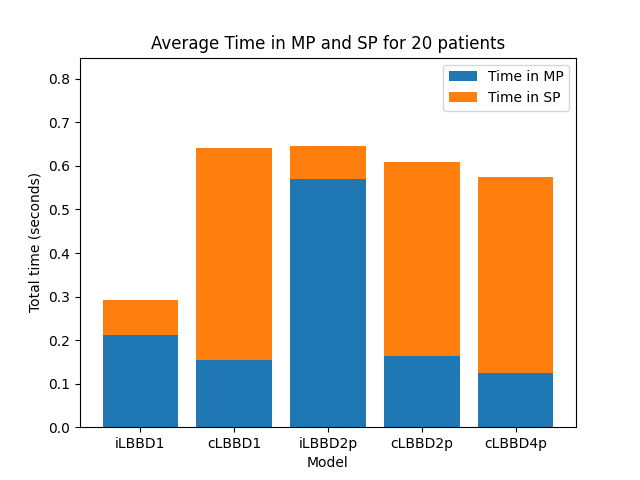
\includegraphics[width=\textwidth]{plots/(20_timeinMPSP).png}
        \caption{$|P|=20$}\label{fig:p=20}
    \end{subfigure}
    \begin{subfigure}[b]{0.35\textwidth}
        \centering
        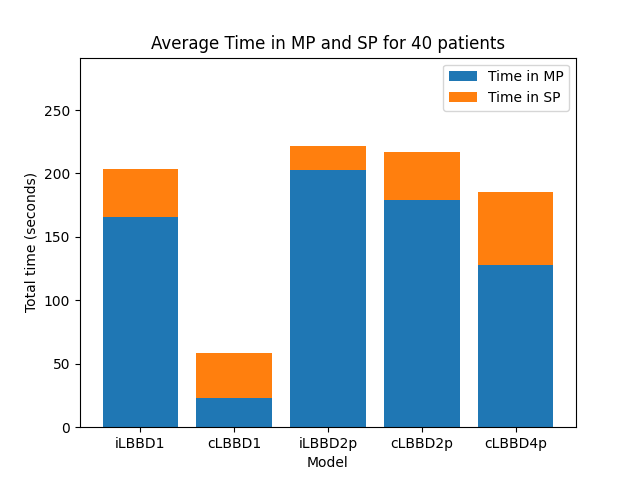
\includegraphics[width=\textwidth]{plots/(40_timeinMPSP).png}
        \caption{$|P|=40$}\label{fig:p=40}
    \end{subfigure}
    \begin{subfigure}[b]{0.35\textwidth}
        \centering
        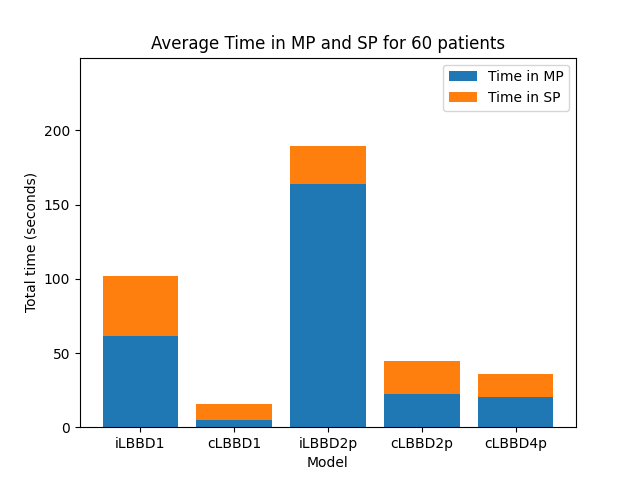
\includegraphics[width=\textwidth]{plots/(60_timeinMPSP).png}
        \caption{$|P|=60$}\label{fig:p=60}
    \end{subfigure}
    \begin{subfigure}[b]{0.35\textwidth}
        \centering
        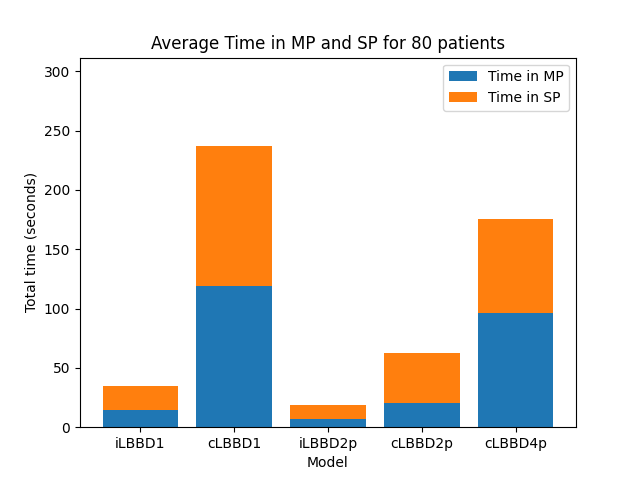
\includegraphics[width=\textwidth]{plots/(80_timeinMPSP).png}
        \caption{$|P|=80$}\label{fig:p=80}
    \end{subfigure}
    \caption{Average time in master problem (MP) and sub problem (SP) for different patient set sizes.}\label{fig:MPSPtime}
\end{figure*}

From Figure~\ref{fig:p=20} we can see that that iterative variants of LBBD spent a high proportion of their time in the master problem and the lazy constraint implementations spent a high proportion of their time in the sub problems. This is expected for the iterative implementation a large amount of time would be spent re-building the master problem branch and bround tree on every iteration. This is expected for the sub problem as we need to solve the sub problems for every incumbent solution, even though it was hoped to be remedied somewhat by caching of sub problems.  

Figure~\ref{fig:p=40} shows that for $|P|=40$ most variants of LBBD including lazy constraint implementations spent large portions of their time in the master problem. This provided some evidence that sub problem implementation was not the main bottleneck for this size of problem, but was in fact the highly optimized Gurobi solver. 

Across all patient set sizes shown in Figure~\ref{fig:MPSPtime} iterative versions consistently spent a high portion of their time in the master problem. Lazy constraint versions seemed to vary with regards to whether they spent more time in master problem or sub problem, this indicates that the relative difficulty of sub problems to master problems was likely highly dependent on the data and not a product of lazy constraints, this was even with using 5 operating rooms which should have influenced the problem to have easier master problems than sub problems\cite{roshanaei2017propagating}.
	\section{Discussion}
	% 15 min time limita
It should be emphasised that because our time constraints are were stricter robustness may have been greatly affected giving different results to the original paper, however we found that our results were already disparate without this factor. For example, the original paper was able to solve with patient sizes up to 100 without ever going over an average run-time of 200 seconds.

% Implementation
We had tr

% Inefficiency of network

% Callbacks not being able to use cuts on incumbents
	\section{Conclusion}
	% Conclusion
We reimplemented a pure MIP and Benders' Decomposition models from~\cite{roshanaei2017propagating}. Models were extended by constructing a new Benders' Cut LBBD4 and by trialling a network model. Implementation was extended by using lazy constraints in Gurobi. Implementations succesfully generated consistent optimal solutions across all models. Implementations generated feasible solutions from observation. Models were able to solve to optimality for only a small patient set size of 20 but were able to scale up to 80 patients when solving to a 1\% gap. We were not able to replicate the efficiency of Benders' Decomposition from the original paper, this was believed to be caused by some sub-optimal implementation used or the difference data generation.  

From our results, the pure MIP model performed the best overall, being the most robust when solving to optimality and being the fastest to solve across all sizes of patient sets when solving to a 1\% gap. The Network model was the least robust when solving to optimality and the slowest when solving to a 1\% gap. Overall, callback implementations performed slightly better than iterative variants.

% Future improvements/work.
Discretizing time further into periods may remedy some of the scaling issues found with all models when solving to optimality, this would sacrifice accuracy for speed, although this can already be done by simply using a larger gap. 

Larger number of patients could be tested to find the limits of the models when solving to a 1\% gap as it was seen that all models were still quite robust up to 80 patients. 

Further algorithmic optimization could be trialled. Caching of sub problems was used to check for identical sub problems but exploratory tests using a more sophisticated caching protocal showed promise, project time constraints and long run-times constrained the collection of more results. The more sophisticated caching methods depend on looking at the sorted set of patients for a given solved sub problem. And the sorted set of patients for the current sub problem. If patient-wise times for the current sub problem are less than or equal to those of a feasible cached sub problem, we know a feasible solution to the current sub problem. Similarly, if the patient-wise time for the current sub problem are greater than or equal to those of an infeasible cached sub problem, we know the current sub problem must be infeasible. The results for this may show great improvement, especially for lazy constraint implementations where similar sub problems are visited often.

	\printbibliography
	\appendix
	\section{Appendix}
	\begin{table*}
    \centering
    \caption{Time taken for each instance when trying to solve to optimality.}
    \begin{tabular}{rrrrrrrrr} \toprule
        seed & $|\mathcal{P}|$ & Pure MIP & Network & iLBBD1 & cLBBD1 & iLBBD2p & cLBBD2p & cLBBD4 \\\midrule
        42     &       20    & 55.621249 &  900     & 4.123265 &  0.949113 & 3.958082 & 0.605675 & 0.654821 \\
       831     &       20    &18.126045 &   900     & 0.296833 &  0.253265 & 0.274671 & 0.416003 & 0.441198 \\
      306       &     20     &2.041458  &   900     & 1.361992 & 2.055692 & 1.106399 & 1.808341 & 1.716485 \\
      542       &     20     &3.000340  &  900     &  0.580737 & 0.504805 & 0.600731 & 0.514555 & 0.520827 \\
        1      &      20     &1.505760  &  900     & 1.181184 & 0.651583 & 1.215210 & 1.055650 & 0.611608 \\\midrule
       42      &      40    &   39.046759 &   &  901.969151 & 900.928267  & 900.922126 &  902.530971 & 901.404782 \\
     831       &     40    & 900.074868 &     &  1171.195916 & 900.966696 & 1605.561038 &  900.273473 & 900.329041 \\
     306       &     40    &  3.928887 &      &     4.428572  &  1.911088  &   4.503378  &  1.910761  &  1.959761 \\
    542       &     40   & 900.199757 &      &  1045.090099  & 901.370528  & 907.687432 &  901.559075 & 900.948533 \\
     1        &    40  &  494.895451  &      &  905.294060 &  905.809085  &  935.405877 & 900.435013 & 904.002700 \\\midrule
     42       &     60 &  900.136048  &       & 902.127126 &  900.441417  & 905.850299 &  903.361533 &  900.170979 \\
     831      &      60 &  900.159431  &      & 912.129558 & 900.112896 & 1183.786823 &  900.232333 &  902.206866 \\
     306      &      60  &  30.804891 &      &  24.459900  & 10.726104  &  34.606863 &  21.455653 &  25.795459 \\
     542      &      60 & 900.154018 &      &  901.279073 & 900.676095 &  919.253635 & 901.173662 & 901.073426 \\
     1        &    60  & 900.127659 &       & 1071.186251 & 900.254857 & 1084.595362 &  900.801214 & 900.983243 \\
     
     \bottomrule
    \end{tabular}
\end{table*}

\begin{table*}
    \centering
    \caption{Gap reached for each instance when trying to solve to optimality.}
    \begin{tabular}{rrrrrrrrr} \toprule
        seed & $|\mathcal{P}|$ & Pure MIP & Network & iLBBD1 & cLBBD1 & iLBBD2p & cLBBD2p & cLBBD4 \\\midrule
        42     &       20 & 0.0 &&    0.0  &   0.0   &   0.0   &   0.0   &   0.0 \\
        831      &      20 & 0.0 &&    0.0  &   0.0  &    0.0   &   0.0   &   0.0\\
        306      &      20 & 0.0 &&    0.0  &   0.0  &    0.0   &   0.0   &   0.0\\
        542      &      20  &0.0 &&    0.0  &   0.0  &    0.0  &    0.0   &   0.0\\
        1       &     20 & 0.0   &&  0.0  &   0.0   &   0.0   &   0.0   &   0.0\\\midrule
       42       &     40&  0.000000 &&    0.0&  0.004805&  0.000000 & 0.011210 & 0.011384\\
       831      &      40 & 0.000136 &&    0.0&  0.007263 & 0.000476&  0.007375&  0.007816\\
        306     &       40 & 0.000000 &&    0.0&  0.000000&  0.000000 & 0.000000&  0.000000\\
       542      &      40&  0.001973  &&   0.0&  0.001876  &0.000000 & 0.001533 & 0.001893\\
         1      &      40 & 0.000000  &&   0.0 & 0.003714 & 0.000000 & 0.003705 & 0.003645\\\midrule
        42       &     60&  0.003867&&  0.00000&  0.004018 & 0.000000 & 0.005890 & 0.005160 \\
        831      &      60&  0.001023&&  0.00000&  0.002758&  0.000024&  0.002752&  0.005001\\
        306      &      60&  0.000000&&  0.00000&  0.000000&  0.000000&  0.000000 & 0.000000\\
        542      &      60 & 0.001695&&  0.00000&  0.003204&  0.000000&  0.006188 & 0.003469\\
        1        &    60 & 0.002548&&  0.00004&  0.002722 & 0.000061 & 0.002733 & 0.002733\\
      \bottomrule
    \end{tabular}
\end{table*}

\begin{table*}
    \centering
    \caption{Objective values when trying to solve to optimality.}
    \begin{tabular}{rrrrrrrrr} \toprule
        seed & $|\mathcal{P}|$ & Pure MIP & Network & iLBBD1 & cLBBD1 & iLBBD2p & cLBBD2p & cLBBD4 \\\midrule
  42      &      20         & -312419.0 &         & -312419.0 &-312419.000000 & -312419.0 & -312419.0 & -312419.0 \\
 831      &      20         & -187989.0  &        &-187989.0 & -187989.000000 & -187989.0 & -187989.0 &-187989.0 \\
  306      &      20       & -220079.0 &           &-220079.0 & -220079.000000 & -220079.0 & -220079.0 & -220079.0 \\
 542       &     20        & -238297.0 &          &-238297.0 & -238297.000000 & -238297.0 & -238297.0 & -238297.0 \\
    1      &      20       & -244112.0 &          &-244112.0 & -244112.002591 & -244112.0  & -244112.0 & -244112.0 \\\midrule
    42       &    40& -503251.0& &-503651.0& -501294.0& -503651.0& -498116.0& -498046.0 \\
    831     &       40& -367748.0&& -368833.0& -366247.0& -368833.0& -366197.0& -366047.0 \\
    306   &         40& -383537.0&& -383537.0& -383537.0& -383537.0& -383537.0& -383537.0 \\
    542   &         40& -412576.0&& -413322.0& -412576.0& -413322.0& -412722.0& -412576.0 \\
    1     &       40& -402834.0&& -403067.0& -401653.0& -403067.0& -401653.0& -401653.0 \\\midrule
    42     &       60 &-741357.0&& -744307.0& -741357.0 &-744307.0& -740007.0& -740542.0 \\
    831   &         60& -654542.0&& -655215.0& -653458.0& -655215.0& -653458.0 &-652005.0\\
    306    &        60& -564312.0&& -564312.0& -564312.0 &-564312.0& -564312.0& -564312.0\\
    542     &       60& -675220.0&& -675400.0& -673288.0& -675400.0& -671849.0& -673117.0\\
    1       &     60 &-602474.0&& -604042.0& -602474.0& -604042.0 &-602474.0& -602474.0\\
    \bottomrule
    \end{tabular}
\end{table*}

\end{document}